\documentclass{article}

\def\ParSkip{} 
\input{../common/ryantibs}
\usepackage{centernot}
\usepackage{cprotect}

\title{Lecture 2: Measures of Dependence and Stationarity \\ \smallskip  
\large Introduction to Time Series, Fall 2024 \\ \smallskip
Ryan Tibshirani}
\date{}

\begin{document}
\maketitle
\RaggedRight
\vspace{-50pt}

Related reading: Chapters 1.3--1.5 of Shumway and Stoffer (SS); Chapters
2.8--2.9 of Hyndman and Athanasopoulos (HA).  

\section{Mean and variance}

\begin{itemize}
\item Given a sequence $x_t$, $t = 1,2,3,\dots$, we define its \emph{mean 
    function} (this is viewed as a function of time) by 
  \[
  \mu_{x,t} = \E(x_t)
  \]
  When it is unambiguous from the context which underlying sequence it refers
  to, we drop the first subscript and simply denote this by $\mu_t$

\item Moreover, we define its \emph{variance function} by
  \[
  \sigma^2_{x,t} = \Var(x_t) = \E[(x_t - \mu_t)^2]
  \]
  Again, when the underlying sequence should be clear from the context, we
  simplify notation and denote this by $\sigma^2_t$

\item The mean and variance functions $\mu_t$ and $\sigma^2_t$ are handy 
  objects, because they tell us about salient features of the time series---the
  drift and spread, respectively, that we should expect over time

\item However, in general, they are not enough to characterize the entire
  distribution of the time series. Why? Two reasons: 

  \begin{enumerate}
  \item In general, the mean and variance are not enough to characterize the
    \emph{marginal} distribution of a single variate $x_t$ along the sequence 

  \item Furthermore, they say nothing about the \emph{joint} distribution of
    two variates $x_s$ and $x_t$ at different times, $s \not= t$. (For example,
    do they tend to go up and down together, or do they tend to repel, or ... ?) 
  \end{enumerate}

  The second of these (joint dependence) we will address soon when we talk about
  auto-covariance and stationarity. The first (mean and variance specifying the 
  distribution) we will revisit later when we talk about Gaussian processes  

\item Before moving on though, let's look at some examples. First, let's
  consider white noise, which recall, refers to a sequence $x_t$, $t =
  1,2,3,\dots$ of uncorrelated random variables, with zero mean, and constant
  variance. Precisely,   
  \begin{gather*}
  \Cov(x_s, x_t) = 0, \quad \text{for all $s \not= t$} \\
  \E(x_t) = 0, \; \Var(x_t) = \sigma^2, \quad \text{for all $t$} 
  \end{gather*}
  So by definition (this one is kind of vacuous), we have mean function $\mu_t =
  0$ and variance function $\sigma^2_t = \sigma^2$, which are constant functions
  (do not vary in time)

\item How about a moving average of white noise, with window length 3? This is 
  \[
  y_t = \frac{1}{3} \Big( x_{t-1} + x_t + x_{t+1} \Big)
  \]
  Its mean function is
  \begin{align*}
  \mu_t &= \E(y_t)  \\
  &= \frac{1}{3} \Big( \E(x_{t-1}) + \E(x_t) + \E(x_{t+1}) \Big) \\ 
  &= \frac{1}{3} ( 0 + 0 + 0 ) \\
  &= 0
  \end{align*}
  Its variance function is
  \begin{align*}
  \sigma^2_t &= \Var(y_t) \\
  &= \frac{1}{9} \Big( \Var(x_{t-1}) + \Var(x_t) + \Var(x_{t+1}) +{} \\
  &\qquad\qquad 2 \Cov(x_{t-1}, x_t) + 2 \Cov(x_t, x_{t+1}) + 2 \Cov(x_{t-1}, 
    x_{t+1}) \Big) \\
  &= \frac{1}{9} ( \sigma^2 + \sigma^2 + \sigma^2 + 0 + 0 + 0) \\
  &= \frac{1}{3} \sigma^2
  \end{align*}
  So its variance is smaller than that of original sequence. In short, smoothing
  reduces variance 

\item This last example might have helped you de-rust on some basic facts about
  expectations and variances. Recall, for constants $a_i$ and random variables
  $x_i$: 
  \begin{gather*}
  \E\bigg( \sum_{i=1}^n a_i x_i \bigg) = \sum_{i=1}^n a_i \E(x_i) \\
  \Var\bigg( \sum_{i=1}^n a_i x_i \bigg) = \sum_{i=1}^n a_i^2 \Var(x_i) + 2
  \sum_{i < j} a_i a_j \Cov(x_i, x_j) 
  \end{gather*}

\item The last rule can be thought of as a special case of the more general
  rule, for constants $a_i,b_j$, and random variables $x_i,y_j$: 
  \[
  \Cov\bigg( \sum_{i=1}^n a_i x_i , \sum_{j=1}^m b_j y_j  \bigg) 
  = \sum_{i,j} a_i b_j \Cov(x_i, y_j)
  \]
  (To be clear, the sum on the right-hand side above is taken over $i =
  1,\dots,n$ and $j = 1,\dots,m$) 

\item Ok, one last example before moving on: let's consider a random walk with
  drift,
  \[
  x_t = \delta + x_{t-1} + w_t
  \]
  for a white noise sequence $w_t$, $t = 1,2,3\dots$.  Recall, we can
  equivalently write this as (assuming we start at $x_0 = 0$):  
  \[
  x_t = \delta t + \sum_{i=1}^t w_i 
  \] 
  From this, we can see that the mean function is 
  \[
  \mu_t = \delta t + \sum_{i=1}^t \E(w_i) = \delta t
  \]
  and the variance function is 
  \[
  \sigma^2_t = \sum_{i=1}^t \Var(w_i) + 2 \sum_{i<j} \Cov(w_i, w_j) = \sigma^2 t 
  \]
  So both the mean and the variance grow over time, proportionally to $t$. 
  Figure \ref{fig:rw} plots example paths over multiple repetitions, for you to
  get a sense of this 

\begin{figure}[p]
\centering
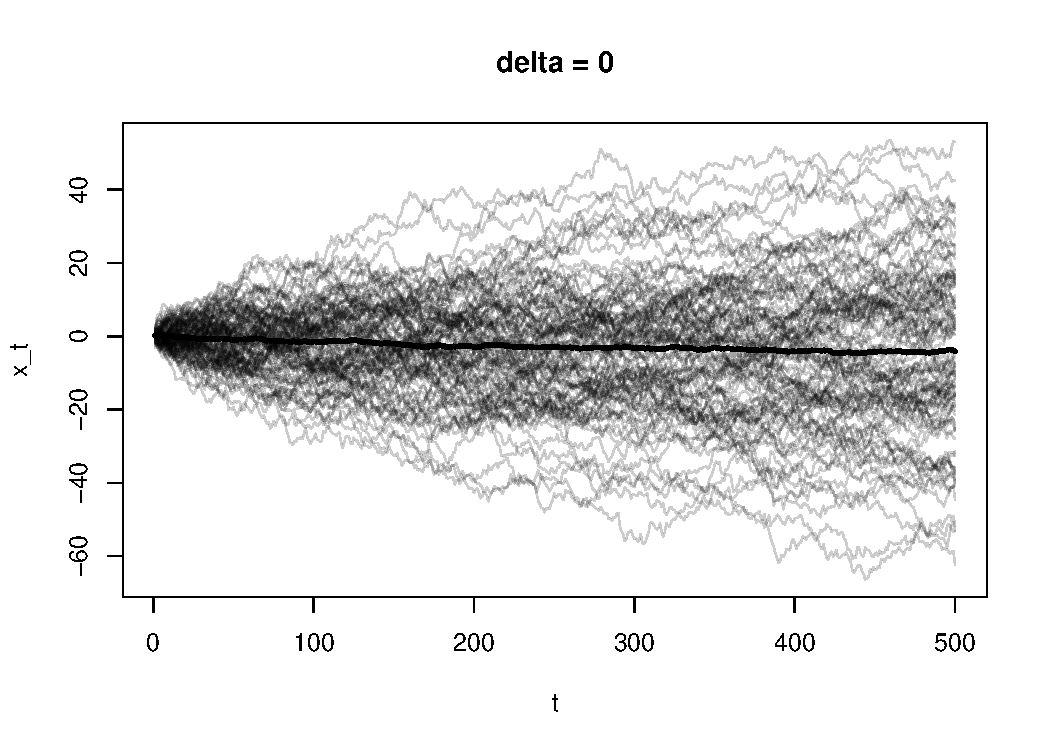
\includegraphics[width=0.875\textwidth]{fig/rw-1.pdf}
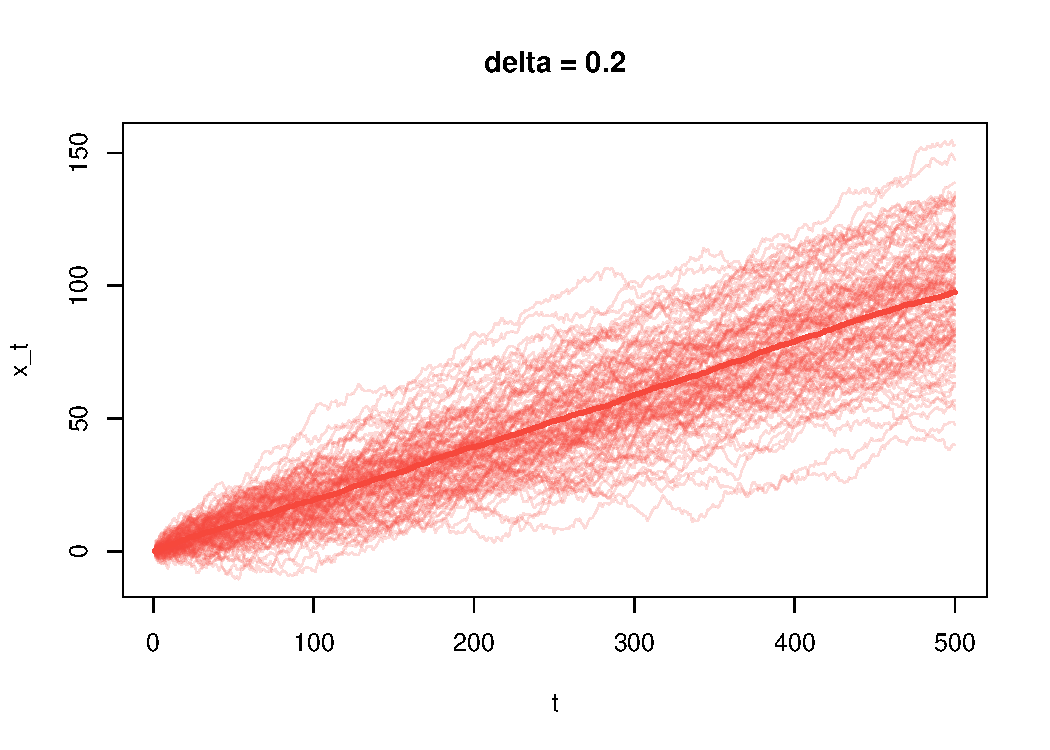
\includegraphics[width=0.875\textwidth]{fig/rw-2.pdf}
\caption{\it Random walk without and with drift, each with 100 sample paths. The
  darker, thicker line in each plot is the sample mean taken at each time point,
  with respect to the 100 repetitions.}
\label{fig:rw}
\end{figure}
\end{itemize}

\section{Covariance and correlation}

\subsection{Auto: one series}

\begin{itemize}
\item The \emph{auto-covariance function} associated with a time series $x_t$,
  $t = 1,2,3,\dots$ is defined as
  \[
  \gamma_x(s,t) = \Cov(x_s, x_t)
  \]
  This is a symmetric function $\gamma_x(s,t) = \gamma_x(t,s)$, for all $s,t$.
  Note that of course $\gamma_x(t,t) = \sigma^2_{x,t}$, the variance
  function. As before, we will drop the subscript when it is clear from the
  context what the underlying sequence is, and simply write $\gamma(s,t)$  

\item The \emph{auto-correlation function} is defined by dividing the
  auto-covariance function by the product of the relevant standard deviations, 
  \[
  \rho_x(s,t) = \frac{\gamma_x(s,t)}{\sigma_{x,s} \, \sigma_{x,t}}
  \]
  which we abbreviate as $\rho(s,t)$ when the underlying sequence is clear from
  the context 

\item By the Cauchy-Schwarz inequality, which states that
  \[
  \Cov(x, y) \leq \sqrt{\Var(x) \Var(y)}
  \]
  for any random variables $x,y$, note that we always have
  \[
  \rho_x(s,t) \in [-1, 1]
  \]
  Typically the auto-correlation will lie strictly in between these limits. 
  (What would a sequence with auto-correlation identically equal to 1 look like?  
  Identically equal to $-1$?) 

\item Broadly speaking, the auto-covariance function measures the \emph{linear}
  dependence between variates along the series. If a series is very smooth, then
  the auto-covariance function will typically be large (and positive when $s,t$
  are close together, but it may be negative when $s,t$ are farther apart). If a 
  series is choppy, then the auto-covariance function will typically be close to
  zero 

\item Recall that uncorrelatedness is not the same as independence! So we can
  have $\gamma_x(s,t) = 0$ for all $s,t$, even if $x_t$, $t = 1,2,3,\dots$ are
  not independent random variables. However, for a Gaussian sequence,
  uncorrelatedness implies independence

\item Let's return to our examples. For white noise, the auto-covariance
  function is identically zero, $\gamma(s,t) = 0$ for all $s \not= t$. Hence the
  same is true of the auto-correlation function

\item For a moving average of white noise, the auto-covariance function
  decreases as the gap between $s$ and $t$ grows. For example, for  
  \[
  y_t = \frac{1}{3} \Big( x_{t-1} + x_t + x_{t+1} \Big)
  \]
  we have
  \begin{align*}
  \gamma(s,t) &= \Cov(y_s, y_t) \\
  &= \Cov \bigg( \frac{1}{3} \Big( x_{s-1} + x_s + x_{s+1} \Big), 
    \frac{1}{3} \Big( x_{t-1} + x_t + x_{t+1} \Big) \bigg) \\
  &=  \sigma^2 \cdot 
  \begin{cases}
  1 / 9 & s = t-2 \\
  2 / 9 & s = t-1 \\
  1 / 3 & s = t \\
  2 / 9 & s = t+1 \\
  1 / 9 & s = t+2 \\
  0 & \text{otherwise}
  \end{cases}
  \end{align*}
  (You can go through each case carefully, and use the formula for the
  covariance of linear combinations given previously.) The auto-correlation
  function simply divides this by $\sigma^2 / 3$, since the variance function is 
  constant, and is hence
  \[
  \rho(s,t) = 
  \begin{cases}
  1 / 3 & s = t-2 \\
  2 / 3 & s = t-1 \\
  1 & s = t \\
  2 / 3 & s = t+1 \\
  1 / 3 & s = t+2 \\
  0 & \text{otherwise}
  \end{cases}
  \]

\item For a random walk (with or without drift), the auto-covariance function
  also decreases as the gap between $s$ and $t$ grows, but has a different 
  structure. Considering 
  \[
  x_t = \delta t + \sum_{i=1}^t w_i
  \]
  we have
  \begin{align*}
  \gamma(s,t) &= \Cov(x_s, x_t) \\
  &= \Cov \bigg( \delta s + \sum_{i=1}^s w_i, \delta t + \sum_{i=1}^t w_i \bigg)
    \\  
  &= \sigma^2 \min\{s, t\}
  \end{align*}
  (To see this more clearly, consider the case where $s<t$ and recognize that 
  the sums above overlap with exactly $s$ white noise variates.) The
  auto-correlation function divides this by the product of the relevant
  variances: 
  \begin{align*}
  \rho(s,t) &= \frac{\sigma^2 \min\{s, t\}}{\sigma \sqrt{s} \cdot \sigma 
              \sqrt{t}} \\  
  &= \frac{\min\{s, t\}}{\sqrt{st}}
  \end{align*}

\item Figure \ref{fig:heatmap} gives a visualization of the auto-correlation
  functions for the moving average and random walk settings. The moving average
  auto-correlation function is presented as a banded matrix (though it is hard
  to see the band since the sequence is of total length $n=500$ and most values
  in the auto-correlation matrix are zero). Importantly, we can see that the
  same pattern persists throughout the whole matrix, and all that matters is the 
  distance to the diagonal. This is an important property that we will revisit
  soon (hint: stationarity). Meanwhile, the random walk auto-correlation
  function does \emph{not} have a pattern that persists throughout, and we can
  see a ``cone'' that grows around the diagonal as time grows 

\begin{figure}[htb]
\centering
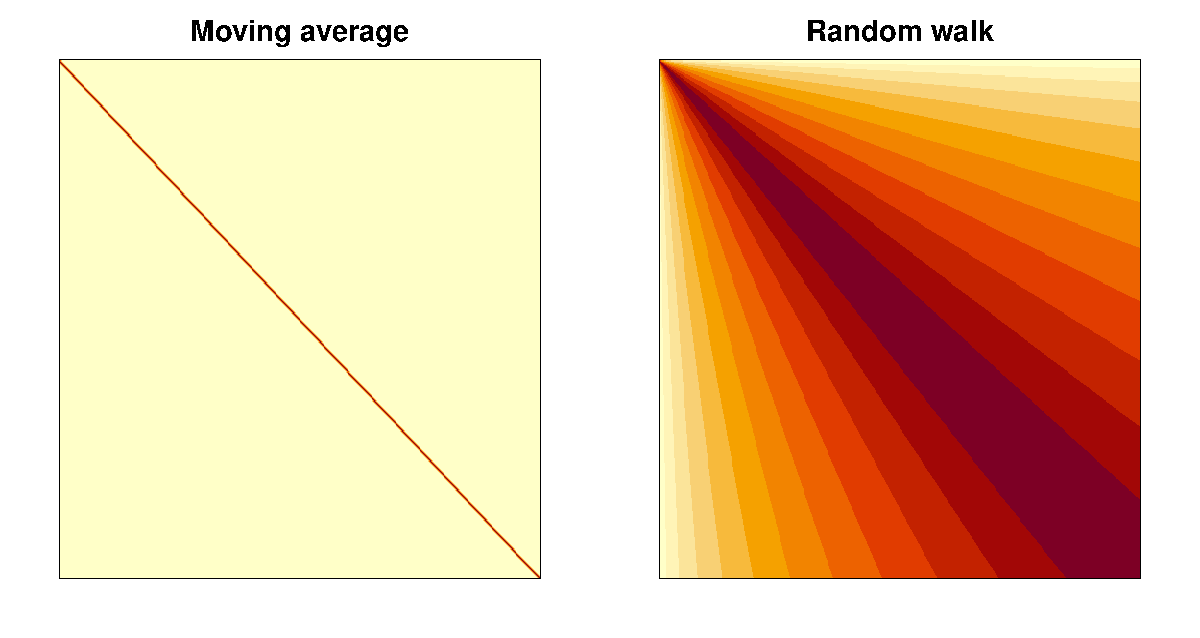
\includegraphics[width=\textwidth]{fig/heatmap-1.pdf}
\caption{\it Heatmaps of the auto-correlation functions for the moving average 
  and random walk examples, for a sequence with $n=500$ time points. The  
  heatmaps are laid out in the same way that we would naturally view a matrix:
  $(s,t) = (1,1)$ is the top left corner, and $(s,t) = (n,n)$ is the bottom
  right (that is, $s$ increases along the rows, and $t$ increases along the
  columns). Yellow reflects a value of zero, and darker red reflects a larger
  value.} 
\label{fig:heatmap}
\end{figure}
\end{itemize}

\subsection{Cross: two series}

\begin{itemize}
\item The \emph{cross-covariance function} associated with two time series $x_t$, 
  $t = 1,2,3,\dots$ and $y_t$, $t = 1,2,3,\dots$ is defined as
  \[
  \gamma_{xy}(s,t) = \Cov(x_s, y_t)
  \]
  This is \emph{not} necessarily a symmetric function, and generically
  $\gamma_{xy}(s,t) \not= \gamma_{xy}(t,s)$. Note that the cross-covariance
  between a time series and itself is simply its auto-covariance, i.e.,
  $\gamma_{xx}(t,t) = \gamma_x(t)$

\item The \emph{cross-correlation function} is defined by diving the
  cross-covariance function by the product of the relevant standard deviations, 
  \[
  \rho_{xy}(s,t) = \frac{\gamma_{xy}(s,t)}{\sigma_{x,s} \, \sigma_{y,t}}
  \]

\item By Cauchy-Schwarz, once again, we know that $\rho_{xy}(s,t) \in [-1,1]$ 

\item Figure \ref{fig:covid-ccf} shows an example of an \emph{estimated} 
  cross-correlation function for Covid-19 cases (the first series $x_s$) and 
  deaths (the second series $y_t$) in California, which are plotted in Figure
  \ref{fig:covid-ts}. We can see that the cross-correlation is plotted as a
  function of ``lag'', which refers to the value $h = s-t$, and appears to be  
  maximized at a lag of $h = -25$ or so. This makes sense, in that we expect
  cases to be highly correlated with deaths several weeks later (this is also
  visually apparent in Figure \ref{fig:covid-ts})

\begin{figure}[p]
\centering
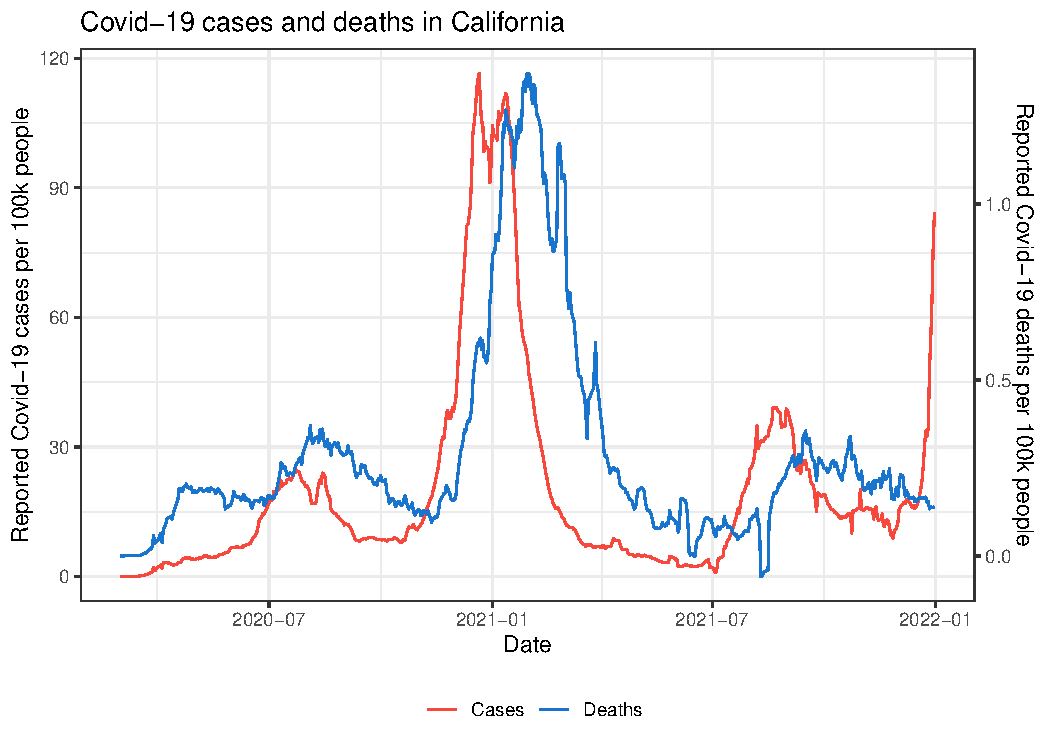
\includegraphics[width=0.85\textwidth]{fig/covid-1.pdf}
\caption{\it Covid-19 cases and deaths, in the state of California.}
\label{fig:covid-ts}

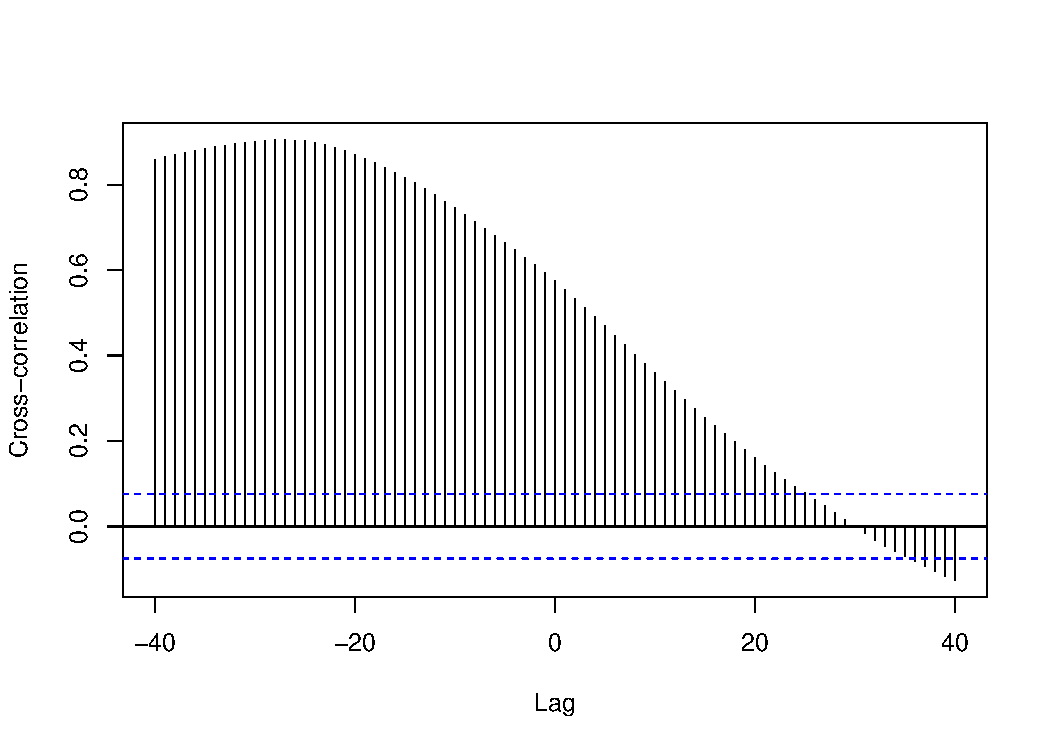
\includegraphics[width=0.875\textwidth]{fig/covid-2.pdf}
\cprotect\caption{\it Cross-correlation function for Covid-19 cases and deaths in
  California, as plotted above. This is estimated by the \verb|ccf()| function 
  in R.}   
\label{fig:covid-ccf}
\end{figure}

\item A bit of nomenclature: we say that cases \emph{lead} deaths, since their
  cross-correlation is maximized at a negative value of $h$, and conversely, 
  deaths \emph{lag} cases  

\item  But wait a minute ... why have we reduced the whole cross-correlation 
  function, which is generically a function of two time indexes $s$ and $t$, to
  be a function of a single number, lag, $h = s-t$? Because that is really the
  only way it is estimable (unless we have more information than the two time
  series at hand). More on this shortly, but next, we'll cover stationarity,
  which will provide the foundation for this estimation strategy in the first
  place 
\end{itemize}

\section{Stationarity}
\def\eqd{\overset{d}{=}}

\subsection{Strong}

\begin{itemize}
\item Stationarity is an important concept in time series. There are actually
  two forms. The first is \emph{strong stationarity} of a time series $x_t$,
  $t = 1,2,3,\dots$, defined by the property:
  \[
  (x_{t_1}, x_{t_2}, \dots, x_{t_k}) \eqd (x_{t_1+\ell}, x_{t_2+\ell}, \dots,
  x_{t_k+\ell}), \quad \text{for all $k \geq 1$, all $t_1,\dots,t_k$, and all
    $\ell$}   
  \]
  Here $\eqd$ means equality in distribution. In other words, strong
  stationarity means that any collection of variates along the series has the
  same joint distribution after we shift the time indices forward or backwards
  in time  

\item As its name suggests, this is a very strong property, in fact, so strong 
  that it'll rarely be useful for most applications. (For example, it is not
  even really possible to assess whether it holds given a single time series)  

\item But before moving on, let's look at some implications of strong 
  stationarity. First, just taking $k=1$, we learn that
  \[
  x_s \eqd x_t, \quad \text{for all $s,t$}
  \]
  In particular, taking the mean of each side above, we see that $\mu_{s,t} =
  \mu_{x,t}$, that is, the mean function must take on a constant value, not
  varying with $t$

\item Second, taking $k=2$, we learn that 
  \[
  (x_s, x_t) \eqd (x_{s+\ell}, x_{t+\ell}), \quad \text{for all $s,t$} 
  \]
  Therefore, taking the covariance of each side above, we see that
  $\gamma_x(s,t) = \gamma_x(s+\ell, t+\ell)$, that is, the auto-covariance
  function must be invariant to shifts, and depend only on the lag $h = s-t$  
\end{itemize}

\subsection{Weak}

\begin{itemize}
\item The second form of stationarity is directly motivated by the implications
  of strong stationarity given at the end of the last subsection. We saw that
  strong stationarity implies that the mean function must be constant, and the
  auto-covariance function must be invariant to shifts. So why not simply
  define a notion based on these two properties?

\item \emph{Weak stationarity} of a time series $x_t$, $t = 1,2,3,\dots$ is
  defined precisely in this way, by the conditions: 
 \begin{gather*}
  \mu_{x,t} = \mu, \quad \text{for all $t$} \\
  \gamma_x(s,t) = \gamma_x(s+\ell, t+\ell), \quad \text{for all $s,t,\ell$}   
  \end{gather*}
  Note that the second condition (take $s=t$) also implies that the variance
  function is constant: $\sigma_{x,t} = \sigma$ for all $t$

\item As we have already discussed, strong stationarity implies weak
  stationarity, but the opposite is not true in general (can you think of an 
  example?). However, it \emph{is} true in the special case that the series is a 
  Gaussian process. We'll summarize this in the next display:
  \begin{align*}
  \text{strong stationarity} &\implies \text{weak stationarity} \\
  \text{strong stationarity} &\centernot\impliedby \text{weak stationarity}   
  \quad \text{(in general)} \\
  \text{strong stationarity} &\impliedby \text{weak stationarity}  
  \quad \text{(for a Gaussian process)} 
  \end{align*}

\item Because the weak form is the much more commonly-used form of stationarity, 
  hereafter, we'll use the term \emph{stationary} to refer to weakly stationary

\item Under stationarity, we will adopt the convention of writing the
  auto-covariance function as a function of just \emph{one} argument, the lag
  $h = s-t$: 
  \[
  \gamma_x(h) := \gamma_x(t, t+h)
  \]
  Here we use $:=$ to emphasize that we are \emph{defining} the quantity on the
  left-hand side, and the value of $t$ on the right-hand side is arbitrary
  (under stationarity, any value of $t$ will result in the same auto-covariance) 

\item Note that, under stationarity, we have $\gamma_x(0) = \sigma^2$, the
  variance (which is constant over time) 

\item Note also that, under stationarity, the auto-correlation function must
  depend only on the lag $h = s-t$, since it is defined as $\rho_x(s, t) =
  \gamma_x(s, t) / ( \sigma_{x,s} \, \sigma_{x,t} )$, where the numerator can  
  only depend on $s-t$, and the denominator must be constant. Hence, under
  stationarity, we will similarly abbreviate the auto-correlation function by:
  \[
  \rho_x(h) := \rho_x(t, t+h)
  \]

\item Let's return to our examples. White noise is clearly stationary---the mean 
  function is identically zero, the variance function is constant, and the
  auto-covariance is zero whenever $s \not= t$. A moving average of white noise 
  is also stationary---the mean function is again identically zero, and the
  auto-covariance derived above is ``symmetric around the diagonal'', i.e., only
  a function of the lag $h = s-t$, which we rewrite below to emphasize this:   
  \[
  \gamma(h) = \sigma^2 \cdot
  \begin{cases}
  1 / 9 & h = \pm 2 \\
  2 / 9 & h = \pm 1 \\
  1 / 3 & h = 0 \\
  0 & \text{otherwise}
  \end{cases}
  \]

\item A random walk is \emph{not} stationary ... even when the drift is zero,
  $\delta = 0$. Why? For one, recall, the variance function is non-constant: it
  increases over time, $\sigma^2_{x,t} = \sigma^2 t$. For another, recall, the 
  auto-covariance function is not symmetric around the diagonal: it is
  $\gamma(s,t) = \sigma^2 \min\{s,t\}$ 

\item Before leaving this section to discuss estimation, we note a
  generalization of stationarity called \emph{trend stationarity}: this means
  that $x_t$, $t = 1,2,3,\dots$ is of the form 
  \[ 
  x_t = \theta_t + w_t
  \]
  where $\theta_t$, $t = 1,2,3,\dots$ is a fixed (nonrandom) sequence and $w_t$,
  $t = 1,2,3,\dots$ is stationary. Intuitively, we think of $x_t$ as being
  ``stationary around the trend $\theta_t$''. While the mean function of such a
  sequence $x_t$ need not be constant (since $\theta_t$ need not be constant),
  it is not hard to check that the auto-covariance function satisfies
  \[
  \gamma_x(s,t) = \gamma_w(s,t)
  \]
  and because the right-hand side is invariant to shifts, so must be the
  left-hand side 
\end{itemize}

\section{Covariance estimation}

\begin{itemize}
\item How do we go about estimating the auto-covariance (or auto-correlation)
  function from a single time series $x_t$, $t = 1,\dots,n$? Well, estimation is 
  not really possible unless we assume stationarity

\item Under this assumption, it is reasonable to consider the \emph{sample 
    auto-covariance function}, defined as 
  \[
  \hat\gamma(h) = \frac{1}{n} \sum_{t=1}^{n-h} (x_{t+h} - \bar{x})(x_t -
  \bar{x}),
  \]
  where \smash{$\bar{x} = \frac{1}{n} \sum_{t=1}^n x_t$} is the sample mean

\item We should note that the sample auto-covariance function is always
  well-defined and can always be computed from data, whether or not the
  stationarity assumption is (approximately) true. But if stationarity is far
  from being true, then the sample auto-covariance function defined above will
  not be very meaningful 

\item Analogously, the \emph{sample auto-correlation function} is defined as 
  \[
  \hat\rho(h) = \frac{\hat\gamma(h)}{\hat\gamma(0)}
  \]
  Note that the denominator here is the sample variance

\item The \verb|acf()| function in R estimates the auto-covariance
  (\verb|type = "covariance"|) or auto-correlation 
  (\verb|type = "correlation"|) function according to the formulas given
  above. An example is given in Figure \ref{fig:speech-acf}, for the speech data
  that we saw in the last lecture, plotted again in Figure
  \ref{fig:speech-ts}. We can see strong patterns here in the sample
  auto-correlation, which makes sense, because the original time series appears
  to be a sequence of repeating short signals   

\begin{figure}[p]
\centering
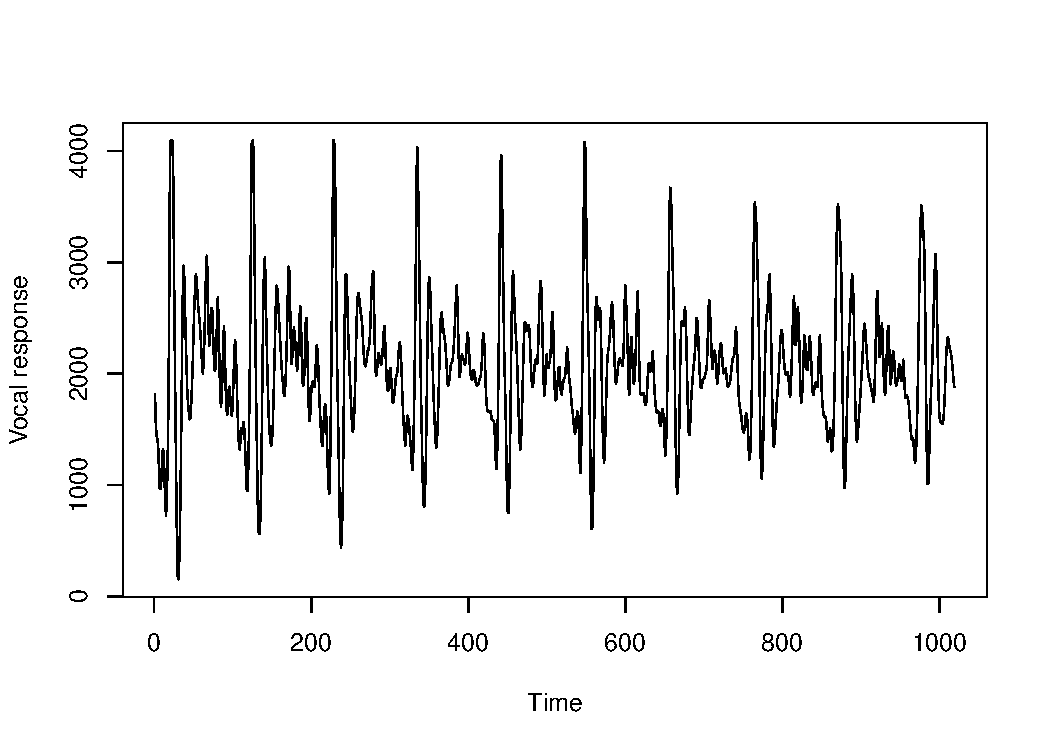
\includegraphics[width=0.875\textwidth]{fig/speech-1.pdf}
\caption{\it Vocal response data measured from the syllable ``aaa $\cdots$ hhh''
  (from SS).}  
\label{fig:speech-ts}

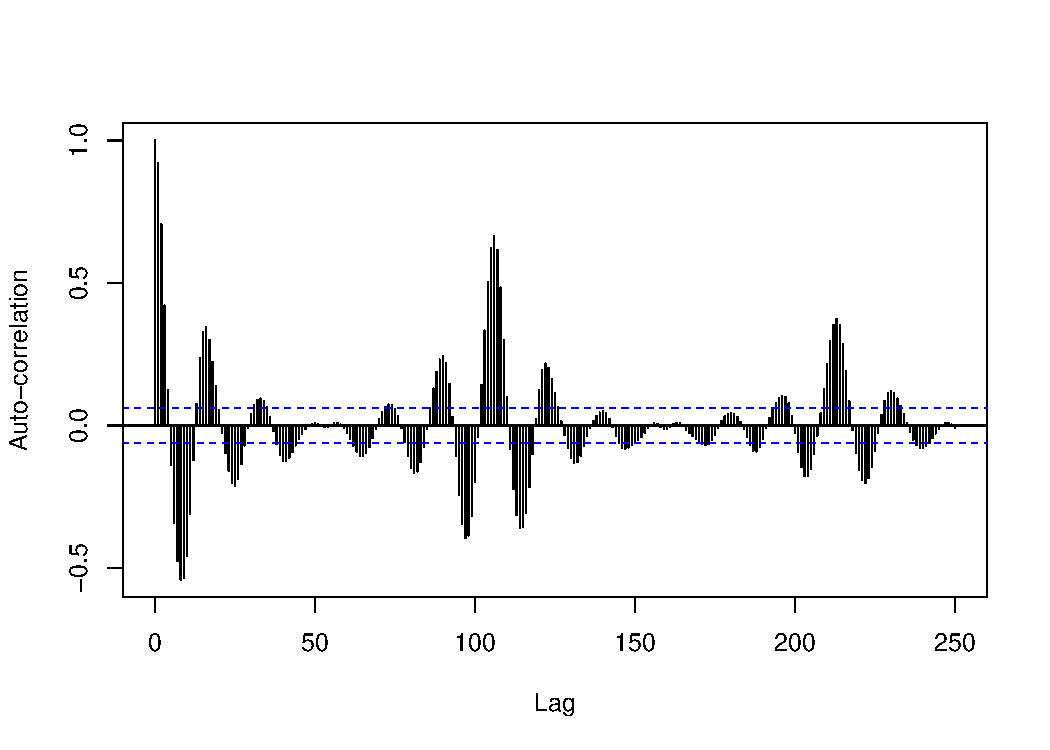
\includegraphics[width=0.875\textwidth]{fig/speech-2.pdf}
\cprotect\caption{\it Auto-correlation function for the speech data, as plotted 
  above. This is estimated by the \verb|acf()| function in R.}   
\label{fig:speech-acf}
\end{figure}

\item The plot produced by \verb|acf()|, by default, also places dotted lines 
  at \smash{$\pm 2/\sqrt{n}$} (where $n$ is the length of the given time
  series). These lines are a tool to hint at statistical significance: under
  some assumptions, for a white noise sequence, the sample auto-correlation at
  any finite lag will be approximately normally distributed with mean zero and
  standard deviation \smash{$1/\sqrt{n}$}, for large $n$. (See Appendix A of SS
  for details)  

\item The \verb|ccf()| function in R estimates the cross-covariance or
  cross-correlation in a manner that is completely analogous to the formulas
  above (for auto-covariance or auto-correlation). These estimates rest on a
  concept called \emph{joint stationarity} between two time series, which you'll
  explore on the homework. Recall, an example of estimated cross-correlation by 
  \verb|ccf()| was already given in Figure \ref{fig:covid-ccf} for the Covid-19
  data  
\end{itemize}

%\section{Pre-whitening}

\section{Gaussian processes}

\begin{itemize}
\item A times series $x_t$, $t = 1,2,3,\dots$ is said to be a \emph{Gaussian
    process} provided that  
  \[
  (x_{t_1}, x_{t_2}, \dots, x_{t_k}) \; \text{has a multivariate Gaussian
    distribution}, \quad \text{for all $k \geq 1$, and all $t_1,\dots,t_k$} 
  \]

\item Recall, if the random vector $(x_{t_1}, x_{t_2}, \dots, x_{t_k})$ has a 
  multivariate Gaussian distribution, then it is defined by a mean vector $\mu
  \in \R^k$ and covariance matrix $G \in \R^{k \times k}$. We denote the
  associated normal distribution by $N(\mu, G)$, and its density is (get ready
  for some linear algebra notation ...): 
  \[
  f(x) = \frac{1}{\sqrt{(2\pi)^k \det G}} \exp \Big( - \frac{1}{2} (x - \mu)^\T
    G^{-1} ( x - \mu ) \Big)  
  \]
  Here $G^{-1}$ is the inverse of the matrix $G$, $\det G$ is its determinant,
  and $(x-\mu)^\T$ is the transpose of the vector $x-\mu$. By convention we
  treat all vectors as column vectors. (If some of this looks foreign to you,
  then you should review your linear algebra notes ... it is pretty darn hard to
  understand aspects of multivariate Gaussians without linear algebra) 

\item For a Gaussian process, the above display describes the density of a
  collection $(x_{t_1}, x_{t_2}, \dots, x_{t_k})$ variates along the sequence,
  but importantly---even though our notation doesn't reflect this, because
  otherwise it would be too cumbersome---the mean vector $\mu$ and covariance
  matrix $G$ here can depend on the time points $t_1,\dots,t_k$. Note that here
  the mean vector $\mu$ has $i\th$ entry 
  \[
  \mu_{x,t_i} = \E(x_{t_i})
  \]
  and the covariance matrix $G$ has, as the element in its $i\th$ row and $j\th$
  column,  
  \[
  \gamma_x(t_i, t_j) = \Cov(x_{t_i}, x_{t_j})
  \]

\item Gaussian processes and weak stationarity are a special combination. If
  $x_t$, $t = 1,2,3,\dots$ is a weakly stationary Gaussian process, then (by
  weak stationarity) the mean vector $\mu$ and covariance matrix $G$ associated
  with $(x_{t_1}, x_{t_2}, \dots, x_{t_k})$ are the same as those associated
  with $(x_{t_1+\ell}, x_{t_2+\ell}, \dots, x_{t_k+\ell})$, for any $\ell$. But
  by Gaussianity this actually implies that  
  \[
  (x_{t_1}, x_{t_2}, \dots, x_{t_k}) \eqd (x_{t_1+\ell}, x_{t_2+\ell}, \dots,
  x_{t_k+\ell}),
  \]
  for any $\ell$, which implies strong stationarity. This proves the claim we
  made above, that for Gaussian processes, weak and strong stationarity are the
  same concept 
\end{itemize}
\end{document}
